\documentclass[a4paper,12pt]{report}


\usepackage[utf8]{inputenc}		% Accents, etc
\usepackage[frenchb]{babel} 		% Francais
\usepackage[T1]{fontenc}			% Encodage de police (césure, accents)
\usepackage{lmodern,textcomp}	% Polices 'Latin Modern' plutôt que 'Computer Modern super'

\usepackage{graphicx}			% Graphiques (images, ...)
\usepackage{amsmath,amssymb}		% Equations
\usepackage[pdftex]{hyperref}	% Lien table des matières

\usepackage{titlesec}			% Chapitres
\titleformat{\chapter}[hang]{\bf\huge}{\thechapter}{2pc}{}

% Taille des sous-titres
\usepackage{titlesec}
\titleformat{\subsection}{\small\bfseries}{\thesection}{1em}{}

% Page de titre du document
\title{Projets de groupe \\ Rapport de reformulation}
\author{J. \bsc{Fanguede}, F. \bsc{Castellane}, G. \bsc{Mahieux}, F. \bsc{Tavares}}
\date{Février 2012}

% Réglages des métadata du PDF
\hypersetup{
pdftitle={Rapport de reformulation},
pdfauthor={J. Fanguede, F. Castellane, G. Mahieux, F. Tavares},
pdfsubject={Projets de groupe 2012},
pdfkeywords={Phelma, Projet, Grenoble, INP, Flyport, OpenPicus}
}

% Début du document
\begin{document}

% Page de titre du document
\maketitle

% Table des matières
\tableofcontents

\chapter*{Introduction}
Les projets de groupe occupent une place importante dans le programme pédagogique de la première année à Phelma. Ils permettent à chacun de travailler en groupe sur une thématique choisie. En outre, ils offrent une première expérience de gestion et de réalisation de projet. 

Ce rapport a pour but de présenter le projet qui a été choisi, de clarifier ses objectifs et d’exposer les solutions techniques envisagées pour sa réalisation.


\chapter{Présentation du projet}
%...

	\section{Problématique et objectifs}
	Le sujet de projet que nous avons choisi est : « voiture radio-commandée en Wi-Fi ». L’objectif du projet est de concevoir le système de commande d’un modèle réduit de voiture, ceci incluant aussi bien l’électronique embarquée que le logiciel de contrôle à distance du véhicule.

Ce projet de robotique a principalement attiré notre attention du fait de sa multi-disciplinarité. En effet, la réalisation d’un tel système implique des compétences à la fois en électronique et en informatique. Or, nous partagions tous un intérêt prononcé pour l’informatique et la programmation.

Ce projet de réalisation d’une voiture radio-commandée en Wi-Fi peut surprendre au premier abord. En effet, une connexion Wi-Fi est plus compliquée à mettre en œuvre, donc plus chère et plus consommatrice qu’une liaison RF classique. Cependant, l’avantage du Wi-Fi est qu’il offre une couche d’abstraction logicielle de haut niveau permettant des communications à double sens entre le contrôleur et la machine à contrôler. C’est-à-dire qu’il est possible de faire remonter facilement des informations à partir de capteurs embarqués sur le véhicule.

C’est donc plus dans une optique de \emph{robot explorateur} que de \emph{jouet radio-commandé} qu’il faut comprendre la démarche que nous avons mené.

	\section{Cahier des charges fonctionnel}
	Le système réalisé devra comporter un certain nombre de fonctionnalités obligatoires à son bon fonctionnement. En particulier, pouvoir contrôler le véhicule d’une manière relativement fluide, offrir une interface de contrôle sur une plate-forme adaptée et disposer d’une autonomie d’au moins quelques minutes. Le cahier des charges fonctionnel est décrit figure~\ref{cdcf}.

Des améliorations pourront par la suite être apportées à l’ensemble afin d’améliorer ses performances et ses fonctionnalités. On pensera notamment, dans la continuité de la section précédente, à des capteurs divers, une caméra, etc. Ces fonctionnalités seront implémentées en fonction de l’avancement du projet et des accords de budget de l’administration.

\begin{figure}[!h]
	\begin{enumerate}
		\item Voiture radio-commandée
		\begin{enumerate}
    			\item Système de connectivité sans-fil
				\begin{enumerate}
    					\item Norme Wi-Fi IEEE 802.11 B/G/N
    					\item Protocoles de communication standards (ex: TCP / IP)
  				\end{enumerate}
    			\item Être contrôlable par un protocole interne
				\begin{enumerate}
    					\item Syntaxe des commandes
  				\end{enumerate}
			\item Rouler à une vitesse satisfaisante
			\item Avoir une autonomie suffisante
    			\item Offrir un retour d’informations au client
				\begin{enumerate}
    					\item Niveau de batterie
					\item Capteurs de proximité
					\item Caméra vidéo
  				\end{enumerate}
  		\end{enumerate}

		\item Logiciel de télécommande
		\begin{enumerate}
    			\item Être implémentable facilement sur une grande variété de plates-formes
				\begin{enumerate}
    					\item Utilisation de protocoles de communication standards (voir 1.a.ii)
  				\end{enumerate}
    			\item Offrir une interface utilisateur conviviale et fonctionnelle
				\begin{enumerate}
    					\item Contrôles adaptés à la plate-forme (ordinateur, smartphone)
  				\end{enumerate}
			\item Pouvoir afficher certaines grandeurs en temps réel (voir 1)
  		\end{enumerate}
	\end{enumerate}

	\caption{Cahier des charges fonctionnel}
	\label{cdcf}
\end{figure}

	\section{Schéma fonctionnel}
	En accord avec le cahier des charges, la figure~\ref{schemafonctionnel} présente rapidement les différentes composantes de l’ensemble et leurs interactions. Celui-ci est composé de deux entités : la télécommande et le véhicule.

Sur la télécommande doit être chargé le logiciel de contrôle qui va être développé. Celui-ci permettra de contrôler le véhicule, de modifier ses réglages réseau et d’observer les signaux en provenance des capteurs. On privilégiera une plate-forme mobile ouverte du type Android.

La voiture devra disposer d’un module Wi-Fi et d’un micro-controlleur programmable, permettant de contrôler les moteurs et de lire les valeurs des capteurs embarqués. L’alimentation (batterie) devra pouvoir alimenter l’ensemble de l’électronique embarquée.

\begin{figure}%[!h]
	\begin{center}
		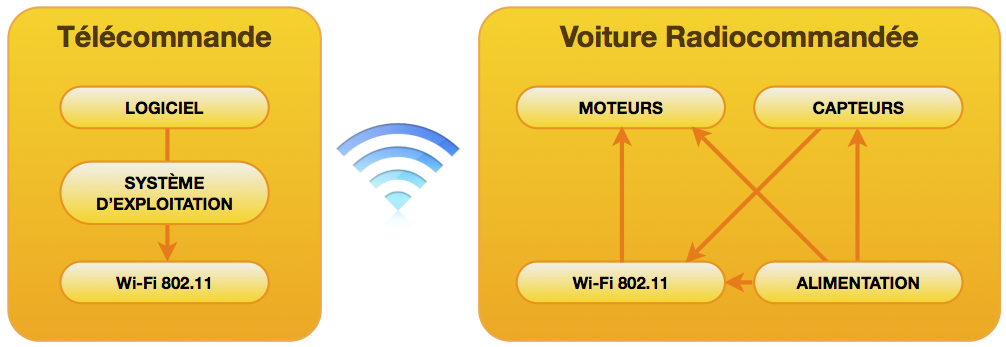
\includegraphics[scale=0.75]{images/schemafonctionnel.png}
	\end{center}
	\caption{Schéma fonctionnel du système}
	\label{schemafonctionnel}
\end{figure}

		\section{Solutions techniques}
		Le pré-découpage du système, présenté précédemment, permet d’envisager des solutions techniques pour chacune de ses composantes.
		
		\subsubsection{La télécommande}
		%\paragraph{La télécommande}
		Celle-ci sera programmée directement sur un système disposant d’une interface Wi-Fi de haut niveau, par exemple un ordinateur sous Linux, Windows ou Mac OS X. Cependant, les exigences de portabilité de la télécommande feront des smartphones sous Android un choix tout à fait pertinent.
		
		\paragraph{}


\end{document}